\section{The control formulation and finite normal periods}\label{sec:reduction}

This appendix gives the precise geometric and analytic setup behind \cref{sec:setting} and
proves the reduction used in \cref{sec:outline-periods}. The first part records the coordinate
formulas, regularity conditions and geometric comparisons. The remaining parts show that a
global minimizer has a finite normal vertex representation.

\subsection{Geometric setup and coordinates}\label{app:setup}

We use the packing densities of \cref{sec:set-packings}. The constructions below follow
Reinhardt, Mahler and Hales, in the form developed in~\cite{HalesVajjha2024}.

\subsubsection{Reinhardt's smoothed octagon}\label{sec:set-octagon}

For $k\in\Z/8$ let
\[
  d_k(x)=1-\bigl(x_0\cos(k\pi/4)+x_1\sin(k\pi/4)\bigr),\qquad x=(x_0,x_1)\in\R^2,
\]
the signed distance from $x$ to the line of the $k$-th side of the regular octagon of inradius
$1$, positive on the side of the origin.

\begin{definition}[The smoothed octagon]\label{def:smoothed-octagon}
Reinhardt's \emph{smoothed octagon} is the set $\Koct$ of the points $x\in\R^2$ such that, for every
$k\in\Z/8$,
\[
  d_k(x)\ge0\qquad\text{and}\qquad
  d_k(x)+d_{k+1}(x)\le\tfrac32-\sqrt2\ \Longrightarrow\ d_{k-1}(x)\,d_{k+2}(x)\ge\tfrac{\sqrt2}{4}.
\]
\end{definition}

The set $\Koct$ is the regular octagon $\{d_k\ge0\}$ with each corner cut off by an arc of a
hyperbola (\cref{fig:octagon}). At the corner between sides $k$ and $k+1$ the hyperbola is
$d_{k-1}d_{k+2}=\sqrt2/4$. Its asymptotes are the lines of the next two sides, $k-1$ and $k+2$, and
it touches sides $k$ and $k+1$ at the two points where $d_k+d_{k+1}=\tfrac32-\sqrt2$: along either
side the product $d_{k-1}d_{k+2}$ is a concave quadratic whose largest value is $\sqrt2/4$, attained
at the point of tangency. Beyond the chord $d_k+d_{k+1}=\tfrac32-\sqrt2$ only the points between the
hyperbola and the origin are kept. Each side of the octagon, of length $2(\sqrt2-1)$, keeps a
straight middle part of length $2-\sqrt2$. The boundary of $\Koct$ is therefore made of eight
segments and eight arcs of hyperbolas, and it is $C^1$, since the arcs leave the segments
tangentially. Mahler~\cite{Mahler1947c} and Ledermann and Mahler~\cite{LedermannMahler1949}
describe the same figure; Hales~\cite{Hales2011} and Hales and Vajjha~\cite[\S7.5]{HalesVajjha2024}
obtain it, in a different linear position, from the control problem below
(\cref{prop:octagon-trajectory,prop:reinhardt-construction}).

\runin{Coordinates for \cref{fig:octagon}.}
(a) Reinhardt's smoothed octagon $\Koct$: the regular octagon of inradius $1$
  (dashed) with its corners cut off; the straight parts of the sides are blue, the arcs of
  hyperbolas orange. (b) The corner $V=(1,\sqrt2-1)$ between side~$0$ ($x_0=1$) and side~$1$
  ($x_0+x_1=\sqrt2$). The hyperbola $d_7d_2=\sqrt2/4$ (thin orange) has the lines of sides~$7$ and
  $2$ as asymptotes, meeting at $C=(1+\sqrt2,1)$, and touches the two sides at
  $T_1=(1,1-1/\sqrt2)$ and $T_2=(\sqrt2-\tfrac12,\tfrac12)$, where $d_0+d_1=\tfrac32-\sqrt2$. The
  arc from $T_1$ to $T_2$ replaces the corner. The straight part of each side has length
  $2-\sqrt2$.

\subsubsection{Critical hexagons and balanced disks}\label{sec:set-balanced}

Let $K$ be centrally symmetric about the origin. Two translates $K+v$ and $K+w$ have disjoint
interiors exactly when $(v-w)/2$ is not an interior point of $K$, so $K+L$ is a packing exactly
when the lattice $\frac12L$ has no nonzero point in the interior of $K$. The densest lattice
packings therefore come from the \emph{critical} lattices of $K$, those of least determinant with
no nonzero interior point. Reinhardt and Mahler described them through hexagons: a critical lattice
has six points $\pm p,\pm q,\pm(q-p)$ on the boundary of $K$, the vertices of an affinely regular
hexagon inscribed in $K$, and a least such hexagon gives a critical lattice
\cite{Reinhardt1934,Mahler1947c}; see \cite[\S2.2]{HalesVajjha2024}. For a worst disk, Reinhardt
showed that the least hexagons form a one-parameter family whose vertices sweep the whole boundary,
and Hales normalized this family as follows.

The \emph{sixth roots of unity} $s_j=(\cos(j\pi/3),\sin(j\pi/3))$, $j\in\Z/6$, satisfy
$s_{j+3}=-s_j$, $s_0+s_2+s_4=0$ and $\det(s_j,s_{j+1})=\sqrt3/2$. A \emph{multi-point} is a map
$j\mapsto\sigma_j\in\R^2$ with the same three properties, and six curves $\sigma_j(t)$ that form a
multi-point at every time are a \emph{multi-curve}. If the points $\sigma_j(t)$ lie on the boundary
of $K$, the hexagon $\sigma_0(t),\dots,\sigma_5(t)$, of area $3\sqrt3/2$, is inscribed in $K$, and
the lattice
\[
  L(t)=2\Z\sigma_0(t)+2\Z\sigma_1(t),\qquad \det L(t)=4\cdot\tfrac{\sqrt3}{2}=\sqrt{12},
\]
contains the six vectors $2\sigma_j(t)$: the translate $K+2\sigma_j(t)$ touches $K$ at
$\sigma_j(t)$.

\begin{definition}[Balanced pair {\cite[Def.~2.4.7]{HalesVajjha2024}}]\label{def:balanced}
A \emph{balanced pair} $(K,\sigma)$ consists of a convex disk $K$ centred at the origin and a
multi-curve $\sigma$ such that each $\sigma_j$ is $C^1$ and regular with Lipschitz derivative, the
curvature $\det(\sigma_j',\sigma_j'')$ is nonnegative almost everywhere, each derivative
$\sigma_j'(t)$ points into the open cone spanned at $\sigma_j(t)$ by $\sigma_{j+1}(t)-\sigma_j(t)$
and $\sigma_{j+1}(t)$ (the \emph{star condition}), and the curves have a common period $6\tf$ over
which each of them traces the boundary of $K$ once. It is in \emph{circle representation} if
$\sigma_j(0)=s_j$ for every $j$.
\end{definition}

\begin{proposition}[{\cite[Thm.~2.2.2]{HalesVajjha2024}}]\label{prop:balanced-density}
If $(K,\sigma)$ is a balanced pair, then $\delta(K)=\area(K)/\sqrt{12}$.
\end{proposition}

For a balanced disk the lattices $L(t)$ thus have the determinant of a densest lattice packing. For
the smoothed octagon the translates $K+L(t)$ are packings, and they form a one-parameter family of
densest packings that slide continuously into one another (\cref{fig:packing}). Baez~\cite{Baez2014}
shows an animation of this family by Greg Egan.


\subsubsection{The control problem}\label{sec:set-control}

Let $(K,\sigma)$ be a balanced pair in circle representation. A multi-point is determined by
$\sigma_0$ and $\sigma_1$, and $\det(\sigma_0,\sigma_1)=\det(s_0,s_1)$, so there is a unique
$g(t)\in\SLtwo$ with $\sigma_j(t)=g(t)s_j$ for every $j$. The matrix $X=g^{-1}g'$ is traceless, the
star condition says that it lies in an open cone, and after a change of time $\det X=1$. The six
curves trace the boundary of $K$ in turn, $\sigma_j(t+\tf)=\sigma_{j+1}(t)$, which reads
$g(t+\tf)=g(t)R$ with $R$ the rotation by $\pi/3$. The convexity of $\sigma_0$ becomes a constraint
on $X'$, which Hales writes with a control in a triangle, and the area of $K$ becomes an integral
of $X$. Hales derived the problem that results in \cite{Hales2011,Hales2017};
\cite[Ch.~3--4]{HalesVajjha2024} gives the derivation in detail.

Write $\ip XY=\tr(XY)$ for the trace form on $2\times2$ matrices, and
\[
  J=\begin{pmatrix}0&-1\\1&0\end{pmatrix},\qquad
  R=\exp(\pi J/3)=\begin{pmatrix}\tfrac12&-\tfrac{\sqrt3}{2}\\[2pt]\tfrac{\sqrt3}{2}&\tfrac12\end{pmatrix}.
\]
The \emph{control simplex} is $\UT=\{u=(u_0,u_1,u_2):u_i\ge0,\ u_0+u_1+u_2=1\}$, with vertices
$\ee_0,\ee_1,\ee_2$. A control $u\in\UT$ has the \emph{control matrix}
\[
  Z_u=\begin{pmatrix}(u_1-u_2)/\sqrt3&(u_0-2u_1-2u_2)/3\\ u_0&(u_2-u_1)/\sqrt3\end{pmatrix}.
\]
For $X=\begin{psmallmatrix}a&b\\c&-a\end{psmallmatrix}$ the \emph{star functions} are
$\rho_0(X)=(c+\sqrt3a)/\sqrt3$, $\rho_1(X)=(c-\sqrt3a)/\sqrt3$ and $\rho_2(X)=-(3b+c)/(2\sqrt3)$.
A \emph{star state} is a traceless matrix $X$ with $\det X=1$ and $\rho_0(X),\rho_1(X),\rho_2(X)>0$.

\begin{definition}[The control problem; {\cite[Problem~3.6.2]{HalesVajjha2024}}]\label{def:control-problem}
Let $T>0$. A \emph{state trajectory} on $[0,T]$ consists of a measurable control
$u:[0,T]\to\UT$, a frame $g:[0,T]\to\SLtwo$ and a state $X$ with values in the star states, such
that
\begin{equation}\label{eq:state}
  g'=gX,\qquad X'=[P_u,X],\qquad P_u=\frac{Z_u}{\ip{Z_u}{X}},
\end{equation}
in the integral sense: the right-hand sides are integrable, and $g$ and $X$ are their indefinite
integrals. It is \emph{admissible} if
\[
  g(0)=I,\qquad g(T)=R,\qquad X(T)=R^{-1}X(0)R .
\]
Its \emph{cost} is
\begin{equation}\label{eq:cost}
  \cost(T,X)=-\frac32\int_0^T\ip{J}{X(t)}\,\dd t .
\end{equation}
\end{definition}

The terminal time $T$ is free, and no regularity of the control beyond measurability is assumed:
this is the class of trajectories in which a minimizer exists \cite[\S6.1]{HalesVajjha2024}, and
the comparison of \cref{sec:set-equivalence} must cover all of it. A global minimizer is defined
accordingly.

\begin{definition}[Global minimizer]\label{def:global-minimizer}
A \emph{global minimizer} is an admissible trajectory $(T,u,g,X)$ such that
$\cost(T,X)\le\cost(T',X')$ for every admissible trajectory $(T',u',g',X')$, with any terminal
time and any measurable control.
\end{definition}

The geometry of the problem is best seen in three coordinates on the star states. The first is a
triple of positive numbers, one for each vertex of the simplex.

\begin{lemma}[Margins]\label{lem:margins}
For a traceless matrix $X$ let $p_i(X)=-\sqrt3\,\ip{Z_{\ee_i}}{X}$, $i\in\Z/3$, be its
\emph{margins}. Then $p_i=2\rho_{2-i}$, and:
\begin{enumerate}[label=\textup{(\roman*)}]
\item a traceless $X$ with $\det X=1$ is a star state if and only if $p_0,p_1,p_2>0$;
\item $p_0p_1+p_1p_2+p_2p_0=4\det X$, which is $4$ on star states;
\item $-\tfrac32\ip JX=\tfrac{\sqrt3}{2}(p_0+p_1+p_2)$, which is at least $3$ on star states;
\item $p_i(R^{-1}XR)=p_{i-1}(X)$.
\end{enumerate}
\end{lemma}

\begin{proof}
For $X=\begin{psmallmatrix}a&b\\c&-a\end{psmallmatrix}$ the margins are $p_0=-(3b+c)/\sqrt3$,
$p_1=2(c-\sqrt3a)/\sqrt3$ and $p_2=2(c+\sqrt3a)/\sqrt3$, which are $2\rho_2$, $2\rho_1$ and
$2\rho_0$; this gives (i). Expanding, $p_0p_1+p_1p_2+p_2p_0=4(-a^2-bc)=4\det X$. Since
$Z_{\ee_0}+Z_{\ee_1}+Z_{\ee_2}=J$, the sum of the margins is $-\sqrt3\ip JX$, which is (iii); and
$(p_0+p_1+p_2)^2\ge3(p_0p_1+p_1p_2+p_2p_0)=12$ gives the lower bound
$\tfrac{\sqrt3}{2}\cdot2\sqrt3=3$. Finally (iv) is a direct computation with the entries of
$R^{-1}XR$.
\end{proof}

By (iii), every state trajectory on $[0,T]$ costs at least $3T$. The second coordinate is a point
of the upper half-plane. For $z=x+iy$ with $y>0$ put
\[
  \Phi(z)=\frac1y\begin{pmatrix}x&-(x^2+y^2)\\1&-x\end{pmatrix}.
\]
Then $\Phi(z)$ is traceless with determinant one, and it is a star state exactly when $z$ lies in
the \emph{star domain}
\[
  \hstar=\{x+iy:\ y>0,\ \abs x<1/\sqrt3,\ x^2+y^2>1/3\},
\]
the ideal triangle with vertices $-1/\sqrt3$, $1/\sqrt3$ and $\infty$; every star state is
$\Phi(z)$ for exactly one $z\in\hstar$ \cite[Thm.~4.4.1]{HalesVajjha2024}. In this coordinate the
margins are
\[
  p_0=\frac{\sqrt3\,(x^2+y^2-1/3)}{y},\qquad p_1=\frac{2(1-\sqrt3x)}{\sqrt3\,y},\qquad
  p_2=\frac{2(1+\sqrt3x)}{\sqrt3\,y},
\]
and each margin vanishes on one side of the ideal triangle. Conjugation by $R$ acts on $\hstar$ by
the M\"obius transformation of $R^{-1}$, which permutes the three sides. The third coordinate, used
from \cref{sec:periods} on, is the triangular form of the state along a piece of constant control.

On an interval where the control is a vertex $\ee_i$, the matrix $P_{\ee_i}$ is a constant multiple
of $Z_{\ee_i}$, the state moves by conjugation by a one-parameter group, and the margin $p_i$ stays
constant (\cref{lem:one-arc}). On such an interval three of the six contact curves trace segments
of the boundary of the disk and the other three trace arcs of hyperbolas. A switch between two
vertices is \emph{forward} if it raises the label by one and \emph{reverse} if it lowers it
(\cref{fig:simplex}). The words of vertex controls are the subject of
\cref{sec:periods,sec:reverse,sec:mixed-runs,sec:short-runs,sec:forward,sec:mixed,sec:terminal}.

\begin{figure}[htbp]
  \centering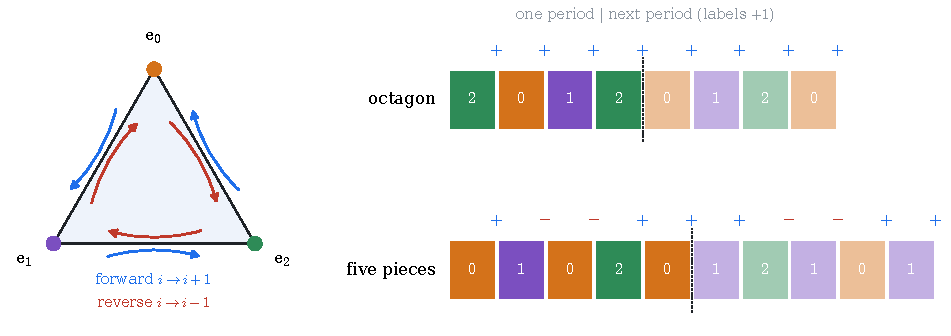
\includegraphics[width=\textwidth]{figures/fig-simplex.pdf}
  \caption{Left: the control simplex $\UT$ with its vertices $\ee_0,\ee_1,\ee_2$; a switch from
  $\ee_i$ to $\ee_{i+1}$ is forward (blue), one from $\ee_i$ to $\ee_{i-1}$ reverse (red). Right:
  two words of vertex labels over one period and the next, with the sign of each switch. The
  terminal condition $X(T)=R^{-1}X(0)R$ raises every label by one from one period to the next, so
  the switch across the seam (dashed) compares the last label of a period with the first label plus
  one. The octagon's word $2\,0\,1\,2$ has four forward switches; the word $0\,1\,0\,2\,0$ has the
  signs $+\,-\,-\,+\,+$. In both cases the signs add up to $1$ modulo $3$
  (\cref{lem:sign-sum}).}
  \label{fig:simplex}
\end{figure}

\subsubsection{The smoothed octagon's trajectory}\label{sec:set-octagon-trajectory}

Let
\[
  y_0=\sqrt{\frac{2\sqrt2-1}{3}},\qquad \tsw=\frac{\log2}{2\sqrt{2\sqrt2-1}},\qquad \tf=4\tsw,
\]
and let $u_{\mathrm{oct}}$ be the control that equals $\ee_2,\ee_0,\ee_1,\ee_2$ on the four
intervals $[m\tsw,(m+1)\tsw)$, $m=0,1,2,3$. The \emph{octagon's density} and \emph{cost} are
\[
  \doct=\frac{8-4\sqrt2-\log2}{2\sqrt2-1}=0.902414\ldots,\qquad
  \Aoct=\sqrt{12}\,\doct=3.126054\ldots .
\]

\begin{proposition}[The octagon's trajectory {\cite[\S7.5]{HalesVajjha2024}}]\label{prop:octagon-trajectory}
There is exactly one state trajectory $(g_{\mathrm{oct}},X_{\mathrm{oct}})$ on $[0,\tf]$ with
control $u_{\mathrm{oct}}$, $g(0)=I$ and $X(0)=\Phi(iy_0)$. It is admissible, its cost is
$\Aoct<\pi$, and it is a Pontryagin extremal (\cref{def:pmp-extremal}). The convex hull
\[
  \KH=\conv\bigcup_{j\in\Z/6}\{g_{\mathrm{oct}}(t)s_j:\ 0\le t\le\tf\}
\]
of its six arcs is a convex disk, symmetric about the origin, of area $\Aoct$ and greatest packing
density $\delta(\KH)=\doct$.
\end{proposition}

\begin{proof}[Sketch]
On a piece of constant vertex control the state equations have explicit solutions
(\cref{lem:one-arc}). From $z_0=iy_0$ the control $\ee_2$ moves the state along
$X(t)=\Phi\bigl((W-1)/\sqrt3+iy_0W\bigr)$, $W=\exp(\sqrt3y_0t)$, and the later pieces are
conjugates of the first by powers of $R$. The choice of $y_0$ makes $\tr(R^{-1}g(\tsw))=\sqrt2$, which
gives $g(\tf)=R$ and $X(\tf)=R^{-1}X(0)R$; uniqueness holds because the right-hand sides are
Lipschitz on each piece. The cost is four times an explicit integral over $[0,\tsw]$, and it equals
$\Aoct$ \cite[\S7.5]{HalesVajjha2024}. The curves $\sigma_j(t)=g_{\mathrm{oct}}(t)s_j$, extended by
$g(t+\tf)=g(t)R$, form a balanced pair with the radial hull of $\sigma_0$, whose area is the cost;
so its density is $\Aoct/\sqrt{12}=\doct$ by \cref{prop:balanced-density}. This radial hull is the
convex hull of the six arcs, which together trace its boundary. Hales and Vajjha prove that the
trajectory is a Pontryagin extremal \cite[Thm.~7.5.6]{HalesVajjha2024}.
\end{proof}

On each of the four pieces the factor $\exp(2\tsw/a)$ of \cref{lem:one-arc}, with $a$ the active
margin, equals $\sqrt2$ (\cref{sec:terminal}). \Cref{fig:contacts} shows the six arcs and the
contact hexagons, and \cref{fig:halfplane} the state in the upper half-plane. The disk $\KH$ is a
linear image of $\Koct$, namely $\KH=A^{-1}\Koct$ with $A=\operatorname{diag}\bigl(1,(2\sqrt2-1)/\sqrt3\bigr)$
(\cref{prop:reinhardt-construction}): Reinhardt's picture compressed vertically by about five per
cent.

\begin{figure}[htbp]
  \centering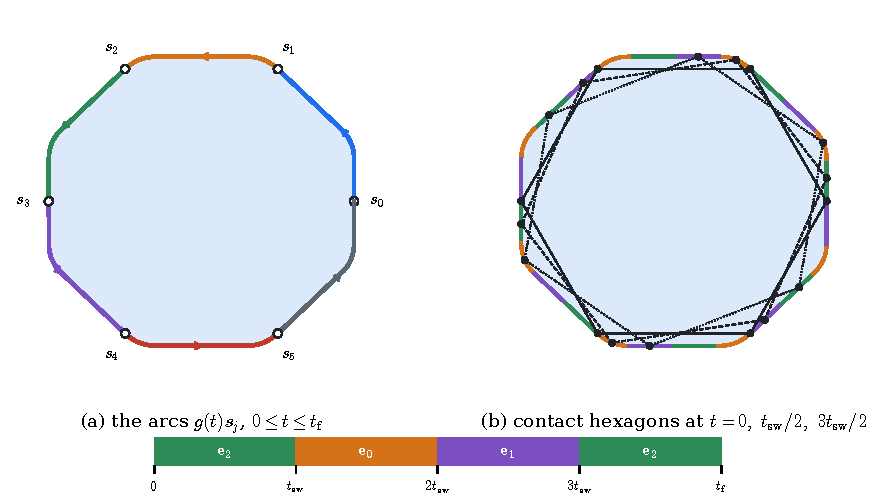
\includegraphics[width=\textwidth]{figures/fig-contacts.pdf}
  \caption{The octagon $\KH$ of the trajectory. (a) As $t$ runs over $[0,\tf]$, the frame
  $g_{\mathrm{oct}}(t)$ carries each sixth root $s_j$ (white) along an arc to $s_{j+1}$; the six
  arcs close up into the boundary of $\KH$, and $\KH$ is their convex hull. (b) The boundary
  coloured by the vertex control that is active when $\sigma_0$ passes there (orange $\ee_0$,
  purple $\ee_1$, green $\ee_2$), and the contact hexagons $\sigma_0(t),\dots,\sigma_5(t)$ at three
  times. Each hexagon has area $3\sqrt3/2$, opposite vertices are antipodal, and consecutive
  vertices span determinant $\sqrt3/2$. Below: the control word $\ee_2\ee_0\ee_1\ee_2$ on
  $[0,\tf]$.}
  \label{fig:contacts}
\end{figure}

\subsubsection{From disks to trajectories and back}\label{sec:set-equivalence}

The reformulation is an equivalence in both directions. One direction realizes a worst disk by an
admissible trajectory of equal cost. The other builds a balanced disk of equal area from every
admissible trajectory of cost below $\pi$, whatever its control. The second direction is what makes
the realization of a worst disk a global minimizer; without it, a cheap trajectory with an
irregular control could undercut every disk.

\begin{proposition}[Realization of a worst disk]\label{prop:realization}
There are a worst disk $K$, a balanced pair $(K,\sigma)$ in circle representation with period
$6T$, and an admissible trajectory $(T,u,g,X)$ with $\sigma_j(t)=g(t)s_j$ for $t\in[0,T]$, such
that
\[
  \cost(T,X)=\area(K)=\sqrt{12}\,\delta(K)\le\Aoct<\pi,\qquad T<\pi/3 .
\]
\end{proposition}

\begin{proof}[Sketch]
Take a worst disk and move it by a linear map, which does not change its density, into Reinhardt's
normal position, in which a least-area circumscribed hexagon has its side midpoints at the sixth
roots of unity. These contact points form the inscribed hexagon used above.
Every boundary point is then a contact point of a least hexagon \cite[\S2.2]{HalesVajjha2024},
and selecting the hexagon whose first contact point has a given polar angle gives six continuous
simple closed curves that trace the boundary. The disk has a unique supporting line at each
boundary point, so its radial parametrization is $C^1$ and regular; reparametrizing by arclength and
then by the clock that makes $\det(g^{-1}g')=1$ gives a balanced pair in circle representation. The
contact map $\sigma_j\mapsto\sigma_{j+1}$ is conjugated by this clock to a translation by one sixth
of the period, which gives $g(t+T)=g(t)R$. The control is read off from the curvatures; where the
three curvatures do not form a nonzero nonnegative vector, which happens only on a null set, any
point of the simplex will do. The area formula for balanced disks gives $\cost=\area(K)$, and
\cref{prop:balanced-density} gives $\delta(K)=\area(K)/\sqrt{12}$. Since $\KH$ is a centrally
symmetric convex disk with $\delta(\KH)=\doct$, the worst disk has $\area(K)\le\Aoct<\pi$, and by
\cref{lem:margins}(iii), $3T\le\cost<\pi$.
\end{proof}

\begin{proposition}[Reverse comparison]\label{prop:reverse-comparison}
Let $(T,u,g,X)$ be an admissible trajectory with $\cost(T,X)<\pi$ and any measurable control.
Then there is a balanced pair $(K,\sigma)$ in circle representation with period $6T$ such that
$\area(K)=\cost(T,X)$ and $\delta(K)=\cost(T,X)/\sqrt{12}$.
\end{proposition}

\begin{proof}[Sketch]
The state of an admissible trajectory is Lipschitz, since the control takes values in a compact set
and the denominator $\ip{Z_u}{X}$ stays away from zero on compact sets of star states; the frame is
$C^1$. Extend the trajectory to all of $\R$ by $G(t+T)=G(t)R$ and $Y(t+T)=R^{-1}Y(t)R$; six copies
close up because $R^6=I$, and the integral equations glue across the seams. Let
$\sigma_j(t)=G(t)s_j$ and let $K$ be the radial hull of $\sigma_0$ over one full period $[0,6T]$.

The terminal condition $g(T)=R$ alone allows the frame to wind around several times, and this is
where the cost bound enters. The reflected first row $(g_{00},-g_{01})$ of the frame turns with
positive angular speed at most $-\ip JX$, so a cost below $\pi$ forces it to turn by exactly
$\pi/3$ over $[0,T]$, with no extra multiple of $2\pi$. The determinant-one identity keeps the first
column $\sigma_0=gs_0$ from ever pointing opposite to the reflected first row, so $\sigma_0$ also
turns exactly once around the origin over $[0,6T]$, and its positive angular speed makes it simple.
The curvature condition of the control makes $\sigma_0$ locally convex, and a simple closed locally
convex curve bounds a convex disk. The other conditions of a balanced pair follow from the state
equations, and the area of the radial hull, $\tfrac12\int_0^{6T}\det(\sigma_0,\sigma_0')$, is the
cost.
\end{proof}

\begin{theorem}[Equivalence]\label{thm:equivalence}
\begin{enumerate}[label=\textup{(\roman*)}]
\item A worst disk exists, and the trajectory of \cref{prop:realization} is a global minimizer of
the control problem, of cost $\sqrt{12}\,\delta_{\min}$.
\item Every global minimizer has cost $\sqrt{12}\,\delta_{\min}$.
\item $\delta(K)\ge\doct$ for every centrally symmetric convex disk $K$ centred at the origin if
and only if $\cost(T,X)\ge\Aoct$ for every admissible trajectory $(T,u,g,X)$.
\end{enumerate}
\end{theorem}

\begin{proof}
Let $(T,u,g,X)$ and $K$ be as in \cref{prop:realization}, and let $(T',u',g',X')$ be any admissible
trajectory. If $\cost(T',X')\ge\pi$, then $\cost(T',X')>\cost(T,X)$. Otherwise
\cref{prop:reverse-comparison} gives a balanced disk $K'$ with
$\cost(T',X')=\area(K')=\sqrt{12}\,\delta(K')\ge\sqrt{12}\,\delta(K)=\cost(T,X)$. This proves (i).
If $(T',u',g',X')$ is another global minimizer, each of the two costs is at most the other, which
gives (ii). For (iii), suppose first that $\delta\ge\doct$ for every such disk. An admissible
trajectory of cost at least $\pi$ costs more than $\Aoct$, and one of cost below $\pi$ costs
$\sqrt{12}\,\delta(K')\ge\Aoct$ by \cref{prop:reverse-comparison}. Conversely, if every admissible
trajectory costs at least $\Aoct$, then the worst disk of (i) has
$\sqrt{12}\,\delta_{\min}=\cost(T,X)\ge\Aoct$, so $\delta(K)\ge\delta_{\min}\ge\doct$ for every such
disk.
\end{proof}

\subsubsection{The compact domain}\label{sec:set-compact}

The star domain $\hstar$ is not compact, and near its three sides some margin is small. Hales and
Vajjha showed that a balanced disk whose area does not exceed the octagon's has its state away
from the sides and from the cusps.

\begin{definition}[The compact domain {\cite[Def.~5.0.1]{HalesVajjha2024}}]\label{def:compact-domain}
$\hstarstar$ is the set of the points $z=x+iy\in\hstar$ with $y\le9/2$,
$(x\mp1/\sqrt3)^2+y^2\ge\tfrac{8}{27}\,y$ for both signs, and $\rho_k(\Phi(z))\ge1/15$ for
$k=0,1,2$. A star state $X$ lies in $\hstarstar$ if $X=\Phi(z)$ with $z\in\hstarstar$.
\end{definition}

The three conditions remove the horoball $y>9/2$ at the cusp $\infty$, its two images under
conjugation by $R^{\pm1}$ (the open disks of radius $4/27$ tangent to the real line at
$\pm1/\sqrt3$), and three neighbourhoods of the sides of $\hstar$. By \cref{lem:margins}, every
margin of a state in $\hstarstar$ is at least $2/15$.

\begin{theorem}[The compact domain {\cite[Thm.~5.0.2]{HalesVajjha2024}}]\label{thm:compact-domain}
The state of every global minimizer lies in $\hstarstar$ at every time. In particular all its
margins are at least $2/15$, at every time and for every vertex, active or not.
\end{theorem}

\begin{proof}
Let $(T,u,g,X)$ be a global minimizer. Its cost is at most that of the octagon's trajectory, which
is $\Aoct<\pi$ (\cref{prop:octagon-trajectory}), so \cref{prop:reverse-comparison} applies: the
cyclic extension of the trajectory is the boundary trajectory of a balanced disk $K$ of area equal
to the cost, with $X=\Phi\circ z$ for a curve $z$ in $\hstar$. Hales and Vajjha prove that if
$z(t_0)$ lies outside $\hstarstar$ at some time, then the area of such a disk is strictly larger than
the area of the smoothed octagon \cite[Thm.~5.0.2]{HalesVajjha2024}: the area is bounded below by
$\sqrt{12}$ times a density function of the single point $z(t_0)$
\cite[Thm.~5.0.6]{HalesVajjha2024}, and this function exceeds $\doct$ off $\hstarstar$. The cost
would then exceed $\Aoct$, the cost of an admissible trajectory, which contradicts minimality.
\end{proof}

\begin{figure}[htbp]
  \centering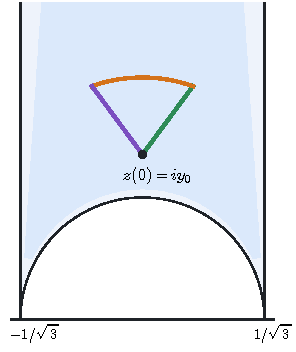
\includegraphics[width=0.62\textwidth]{figures/fig-halfplane.pdf}
  \caption{The star domain $\hstar$ (light), bounded by the lines $x=\pm1/\sqrt3$ and the circle
  $x^2+y^2=1/3$, and the compact domain $\hstarstar$ (darker; its cut at $y=9/2$ lies above the
  frame). The curve is the state $z(t)$ of the octagon's trajectory, $X(t)=\Phi(z(t))$, over three
  periods $[0,3\tf]$, after which it returns to $z(0)=iy_0$; it is coloured by the active vertex
  control as in \cref{fig:contacts}. The curve stays in $\hstarstar$, so every margin along it
  exceeds $2/15$.}
  \label{fig:halfplane}
\end{figure}

\subsubsection{Notation}\label{sec:set-notation}

\Cref{tab:notation} lists the symbols that are used in more than one section. Symbols that belong
to a single case are introduced where they are used.

\begin{longtable}{@{}p{0.22\textwidth}p{0.58\textwidth}p{0.12\textwidth}@{}}
\caption{Notation.}\label{tab:notation}\\
\toprule
Symbol & Meaning & Where\\
\midrule
\endfirsthead
\toprule
Symbol & Meaning & Where\\
\midrule
\endhead
\bottomrule
\endfoot
$\delta(K)$, $\delta_L(K)$ & greatest packing density, greatest lattice packing density & \S\ref{sec:set-packings}\\
$\delta_{\min}$ & least $\delta(K)$ over centrally symmetric convex disks & \S\ref{sec:set-packings}\\
$\Koct$, $\KH$ & Reinhardt's smoothed octagon; the octagon of the trajectory & \S\ref{sec:set-octagon}, \S\ref{sec:set-octagon-trajectory}\\
$d_k(x)$ & distance to the line of the $k$-th side of the regular octagon & \S\ref{sec:set-octagon}\\
$s_j$, $\sigma_j(t)$ & sixth roots of unity; contact curves $g(t)s_j$ & \S\ref{sec:set-balanced}\\
$\ip XY$ & the trace form $\tr(XY)$ & \S\ref{sec:set-control}\\
$J$, $R$ & rotation generator; rotation by $\pi/3$ & \S\ref{sec:set-control}\\
$\UT$, $\ee_i$ & control simplex and its vertices, $i\in\Z/3$ & \S\ref{sec:set-control}\\
$Z_u$, $P_u$ & control matrix; $Z_u/\ip{Z_u}{X}$ & \S\ref{sec:set-control}\\
$g$, $X$, $T$ & frame in $\SLtwo$, star state, terminal time & \S\ref{sec:set-control}\\
$\cost(T,X)$ & the cost $-\tfrac32\int_0^T\ip JX$ & \S\ref{sec:set-control}\\
$\rho_i$, $p_i$ & star functions; margins $p_i=2\rho_{2-i}$ & \S\ref{sec:set-control}\\
$\Phi(z)$, $\hstar$, $\hstarstar$ & the state of $z=x+iy$; star domain; compact domain & \S\ref{sec:set-control}, \S\ref{sec:set-compact}\\
$\doct$, $\Aoct$ & $(8-4\sqrt2-\log2)/(2\sqrt2-1)$ and $\sqrt{12}\,\doct$ & \S\ref{sec:set-octagon-trajectory}\\
$y_0$, $\tsw$, $\tf$ & data of the octagon's trajectory & \S\ref{sec:set-octagon-trajectory}\\
$\Lambda_1$, $\Lambda_R$, $\lambda$ & costates and cost multiplier & \S\ref{sec:reduction}\\
$H$, $H_i$ & Hamiltonian; vertex Hamiltonians & \S\ref{sec:reduction}\\
$N$, $\tau_k$, $i_k$ & pieces per period, switching times, labels & \S\ref{sec:reduction}\\
$a_k$, $q_k$ & active margin and factor of piece $k$ & \S\ref{sec:periods}\\
$\varepsilon_k$ & sign of the switch after piece $k$: $+1$ forward, $-1$ reverse & \S\ref{sec:periods}\\
$s_k$, $K_k$ & $a_k+a_{k+1}$ and $a_k^2+4$ & \S\ref{sec:periods}\\
$T_i(q)$ & tangent factor of a piece with label $i$ & \S\ref{sec:periods}\\
$\cls R$, $\cls F$, $\cls{M1}$, $\cls{M2}$, $\cls{M3}$ & the five classes of sign sequences & \S\ref{sec:periods}\\
$\alpha_j$, $\beta_j$, $\chi_j$ & costate coordinates; $\chi_j=2\alpha_j+\beta_j=p_jH_j$ & \S\ref{sec:periods}\\
$U$, $\mu_j$, $\gamma^2$, $\kappa$ & normal multiplier, its margins, the Casimir $\det U$, $\kappa=\sqrt{12\gamma^2}$ & \S\ref{sec:periods}\\
$y_k$, $d_k$, $e_k$ & switch vectors, switch norms, cross pairings & \S\ref{sec:periods}\\
\end{longtable}
